\documentclass[12pt,a4paper]{article}
\usepackage[utf8]{inputenc}
\usepackage{amsmath}
\usepackage{amsfonts}
\usepackage{amssymb}
\usepackage{placeins}
\usepackage{cmap} % для кодировки шрифтов в pdf
\usepackage[T1]{fontenc}
\usepackage{hhline}
\usepackage[unicode]{hyperref}
\usepackage{multirow}
\usepackage{array}
\usepackage{amsmath}
\usepackage{bm}
\usepackage{textcomp}
\usepackage[russian]{babel}
\usepackage{graphicx} % для вставки картинок
\usepackage{amssymb,amsfonts,amsmath,amsthm} % математические дополнения от АМС
\usepackage{indentfirst} % отделять первую строку раздела абзацным отступом тоже
% Поля
\usepackage{geometry}
\geometry{left=2cm}
\geometry{right=1.5cm}
\geometry{top=2.4cm}
\geometry{bottom=2.cm}

%%%%%%%%%%%%%%%%%%%%%%%%%%%%%%%     

\linespread{1.5} % полуторный интервал
\frenchspacing

\begin{document}
	
	\begin{titlepage}
		
		\begin{center}
			\begin{large}
				Санкт-Петербургский Политехнический университет\\ Петра Великого\\
				Институт прикладной математики и механики\\
			\end{large}
			\vspace{0.2cm}
			Высшая школа прикладной математики и вычислительной физики\\
			
		\end{center}
		
		\vspace{3cm}
		\begin{center}
			\textbf{Отчёт\\ по лабораторной работе 8\\ по дисциплине\\ "математическая статистика"}
		\end{center}
		
		\vspace{3cm}
		\vbox{%
			\hfill%
			\vbox{%0
				\hbox{Выполнил студент:}%
				\hbox{\break}
				\hbox{Аникин Александр Алексеевич,}%
				\hbox{группа 3630102$\backslash$80201}%
				\hbox{\break}
				\hbox{\break}
				\hbox{Проверил:}
				\hbox{\break}
				\hbox{к.ф.-м.н., доцент}
				\hbox{Баженов Александр Николаевич}
			}%
		} 
		\vfill
		
		\begin{center}
			Санкт-Петербург\\2021
		\end{center}
		
	\end{titlepage}
	\tableofcontents
	\newpage
	
	\listoffigures
	\newpage
	
	\listoftables
	\newpage	
	
	\section{Постановка задачи}
	Провести дисперсионный анализ с применением критерия Фишера по данным регистраторов для одного сигнала (содержит 1024 элемента). Определить области однородности сигнала, переходные области, шум/фон.
	\newpage
	
	\section{Теория}
		\subsection{Критерий Фишера}
			\subsubsection{Внутригрупповая дисперсия}
			Внутригрупповая дисперсия:
			\begin{equation}
				s_{IntraGroup}^2=\frac{1}{k}\sum_{i=1}^{k}s_i^2 = 	\frac{1}{k}\sum_{i=1}^{k}\frac{\sum_{j=1}^{n}(x_{ij}-\overline{X})^2}{k-1},
			\end{equation}
			$\overline{X}$ – среднее для части выборки, $k$ – количество частей выборки,
			$n$ – количество элементов в рассматриваемой части выборки.
			Внутригрупповая дисперсия является дисперсией совокупности и
			рассматривается как среднее значение выборочных дисперсий
			
			\subsubsection{Межгрупповая дисперсия}
			Межгрупповая дисперсия:
			\begin{equation}
				s_{InterGroup}^2 = \frac{k}{k-1}\sum_{i=1}^{k}(\overline{X}_i-\overline{X})^2,
			\end{equation}
			где $\overline{X}_i$ – среднее значение $i$-ой подвыборки, $\overline{X}$ –
			среднее значение средних значений подвыборок.
			
			\subsubsection{Критерий Фишера}
			Критерий Фишера:
			\begin{equation}
				F = \frac{s_{InterGroup}^2}{s_{IntraGroup}^2}
			\end{equation}
	\newpage
	
	\section{Реализация}
	Лабораторная работа выполнена на языке Python 3.8 с помощью загружаемых пакетов MatPlotLib, NumPy. Исходный код лабораторной работы находится на GitHub репозитории.
	\newpage
	
	\section{Результаты}
	\begin{figure}[hpt]
		{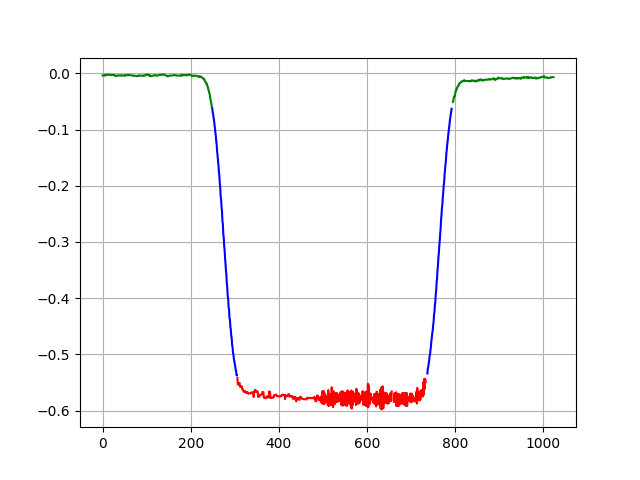
\includegraphics[width=1\linewidth]{../plots/plot.png}}
		\caption{График сигнала с разбиением на области}
	\end{figure}

	\begin{figure}[hpt]
		{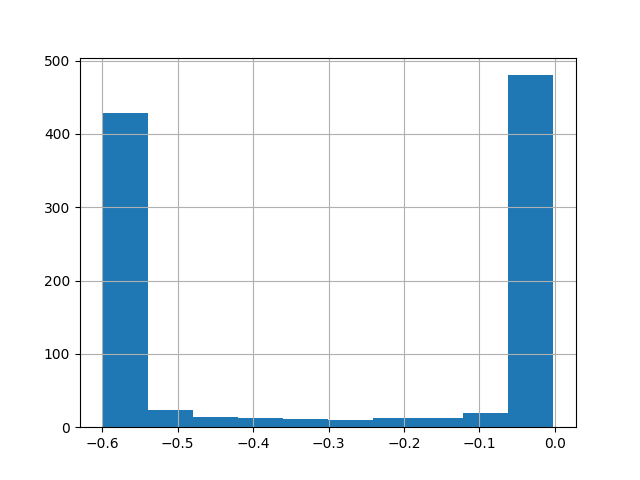
\includegraphics[width=1\linewidth]{../plots/hist.png}}
		\caption{Гистограмма сигнала}
	\end{figure}
	\FloatBarrier
	\newpage
	\begin{table}[hpt]
		\begin{center}
			\begin{tabular}{|c|c|c|c|}
				\hline
				Промежуток & Тип & Количество разбиений & Критерий Фишера \\ \hline
				1 & Фон & 7 & 0.0571 \\ \hline
				2 & Переход & 6 & 66.8766\\ \hline
				3 & Сигнал & 8 & 0.1285 \\ \hline
				4 & Переход & 6 & 65.3247 \\ \hline
				5 & Фон & 7 & 0.3202 \\ \hline
			\end{tabular}
		\end{center}
	\caption{Характеристики областей сигнала}
	\end{table}
	\FloatBarrier
	
	Критерий Фишера в областях фона и сигнала находится в окрестности 1; в областях перехода критерий много больше 1. Остюда можно сделать вывод, что промежутки "фон" и "сигнал" однородны, а промежутки "сигнал" - неоднородны.

	
	\clearpage
	\newpage	
	\begin{thebibliography}{1}
		\addcontentsline{toc}{section}{\bibname}
		\bibitem{maksimov}  Максимов Ю.Д. Математика. Теория и практика по математической статистике. Конспект-справочник по теории вероятностей : учеб. пособие /
		Ю.Д. Максимов; под ред. В.И. Антонова. — СПб. : Изд-во Политехн.
		ун-та, 2009. — 395 с. (Математика в политехническом университете).
		
	\end{thebibliography}
\end{document}